\begin{frame}[fragile]{Metrics for proteins}

\vspace{-0.3in}
\begin{center}
\begin{tikzpicture}
%\node at (0,0) {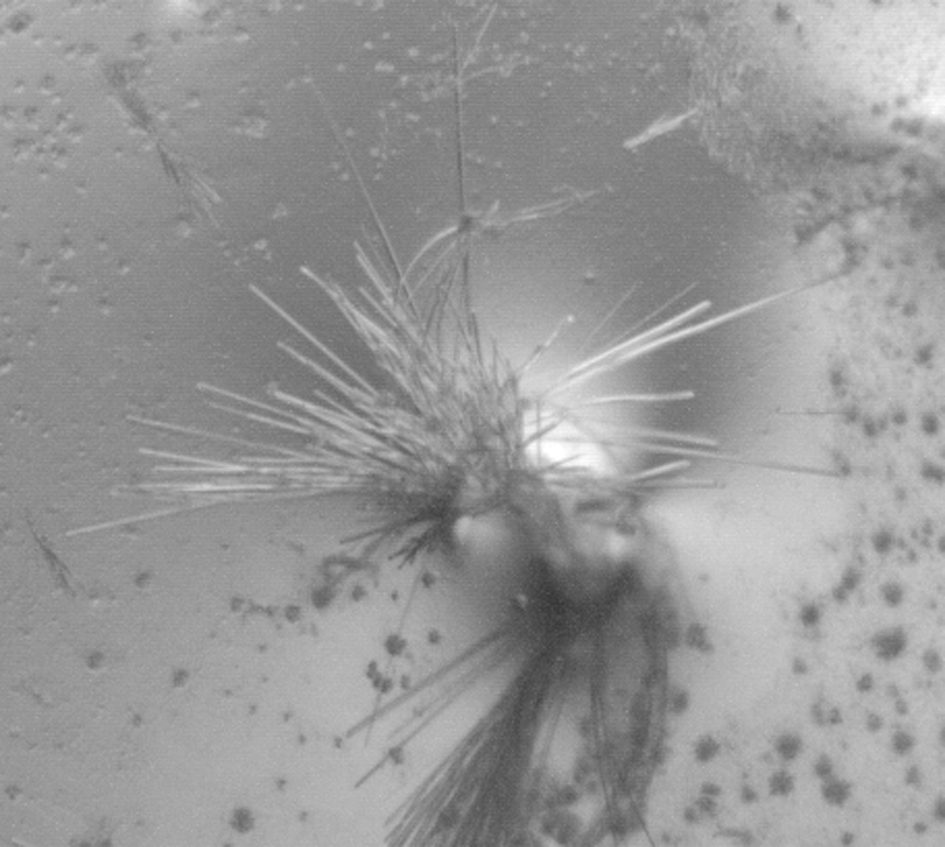
\includegraphics[width=4cm]{slides/covertree/xrayprotein}};
\node at (0,0) {\includegraphics[width=4cm]{img-presentation/Lignin1_0}};
\node at (6,0) {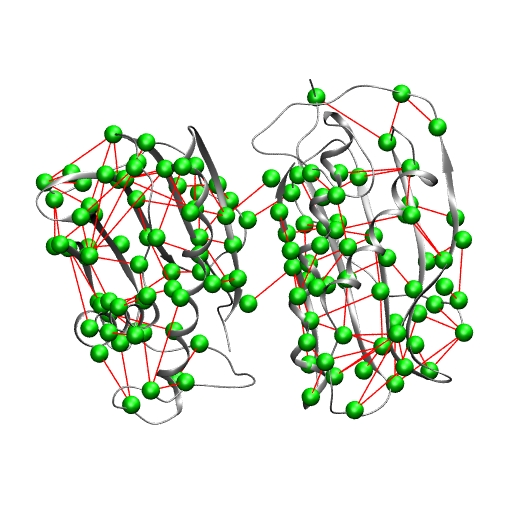
\includegraphics[width=4cm]{slides/covertree/ProteinGraphs}};

\draw[->,line width=4pt] (2.75,0) -- (3.75,0);
\end{tikzpicture}
\end{center}

\vspace{-0.2in}

%The protein databank contains information on $\sim$100,000 proteins
%
%\vspace{0.1in}
Protein structure (and hence function) can be modeled as a graph

\vspace{0.1in}
The random walk graph kernel is a commonly used protein metric

\vspace{0.1in}
This is an \emph{expensive} metric, taking time $O(v^3)$

\vspace{0.1in}
(Vishwanathan \emph{et. al.}, 2010)

\vspace{0.15in}
{\tiny
images from: \url{http://www.lunenfeld.ca}, and \url{http://vishgraph.mbu.iisc.ernet.in/GraProStr/}
}

\end{frame}


